%%%%%%%%%%%%%%%%%%%%%%%%%%%%%%%%%%%%%%%%%%%%%%%%%%%%%%%%%%%%%%%%%%%%
% Authors: A. Herrera, M. Morales, M. Ruíz
% Tittle: Tryton
% 							 DDSI 2017
%%%%%%%%%%%%%%%%%%%%%%%%%%%%%%%%%%%%%%%%%%%%%%%%%%%%%%%%%%%%%%%%%%%%

%!TEX root = ../tryton.tex

\section{Funcionalidad}

    \subsection{Características}

    \begin{frame}{Características}
        \fontsize{10}{11}\selectfont
        \begin{columns}
        \column{0.6\textwidth}
    	\begin{itemize}
    		\item Diseño en 3 capas
    			\begin{itemize}
    				\item Cliente Tryton
    				\item Servidor Tryton
    				\item Base de Datos
    			\end{itemize}
    		\item Módulos
            \item Búsqueda de la perfección
			\begin{itemize}
                \item Documentación dinámica
                \item Registros históricos
				\item Búsqueda global de términos
				\item WebDAV, CalDAV
			\end{itemize}
            \item Evolución
                \begin{itemize}
                    \item Fácil Migración
                    \item Dos actualizaciones anuales
                \end{itemize}
    	\end{itemize}
        \column{0.6\textwidth}
        \begin{itemize}
            \item Multiplataforma
            \item Conectividad
                \begin{itemize}
                    \item Cliente de escritorio
                    \item Cliente web
                    \item Dispositivos Android
                \end{itemize}
        \end{itemize}
        \begin{center}
        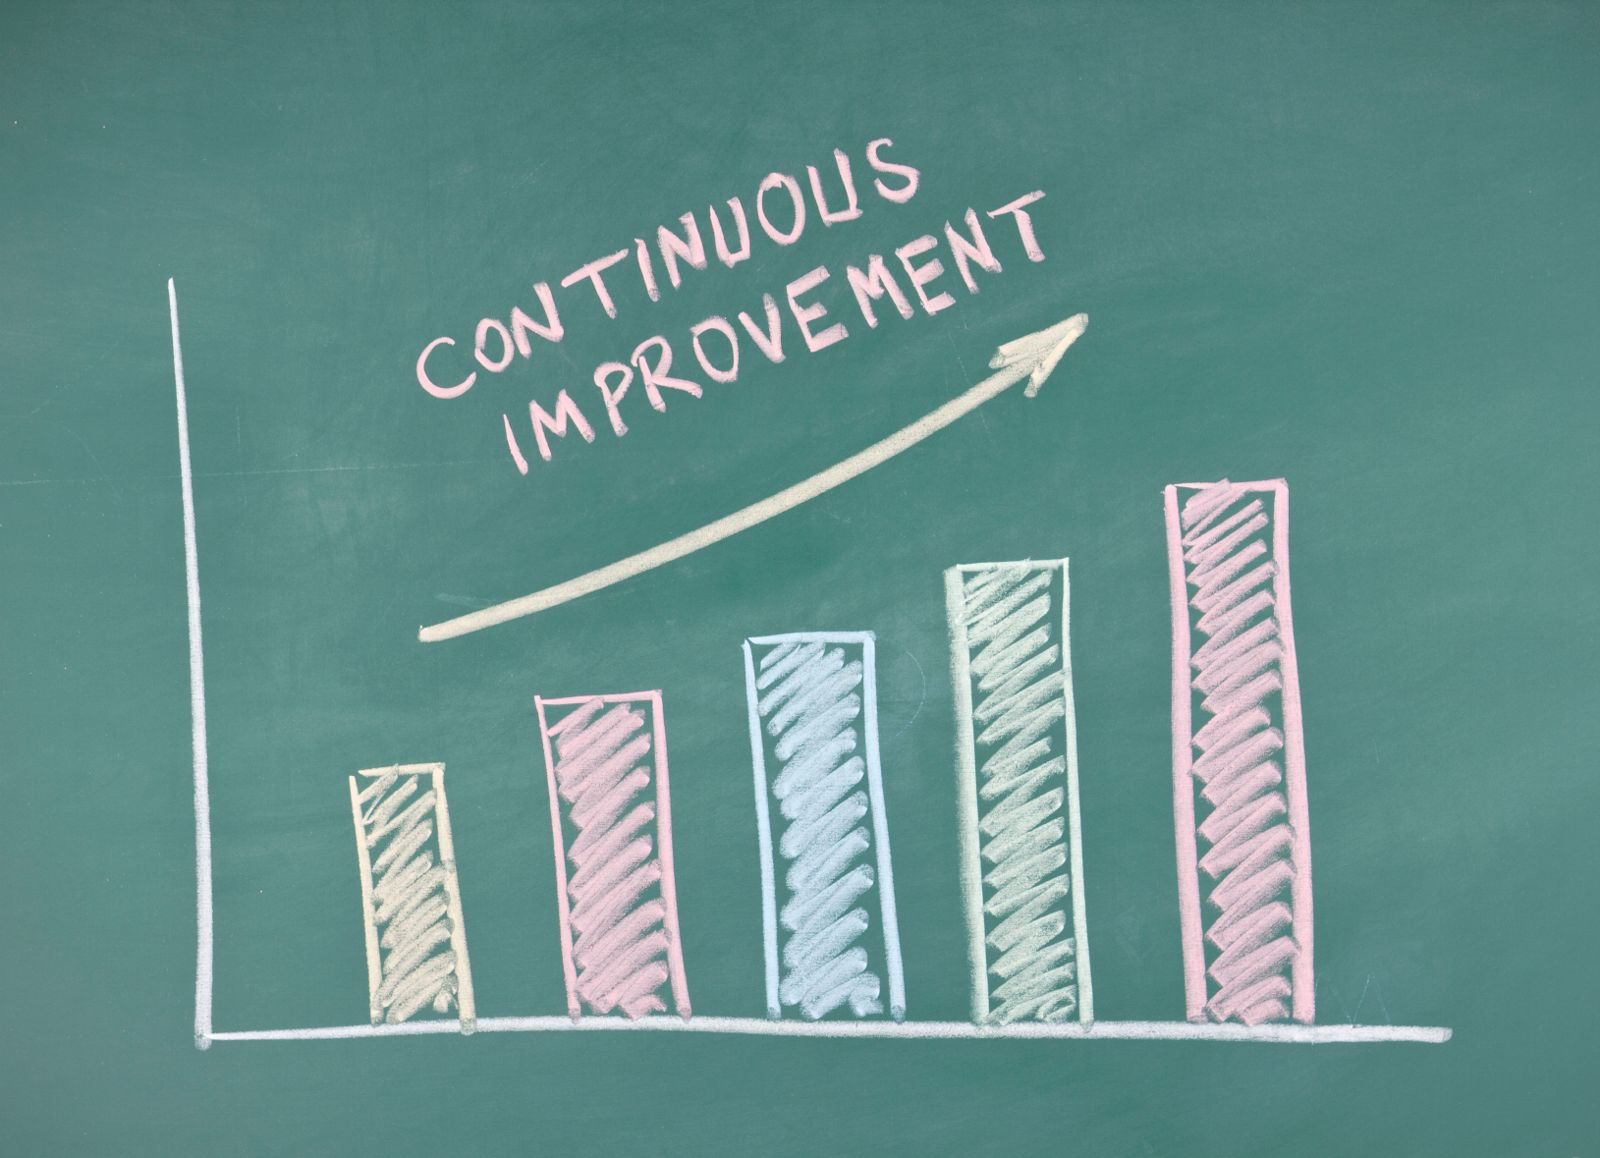
\includegraphics[width=0.8\textwidth]{./Images/improvement.jpg}
        \end{center}
        \end{columns}
    \end{frame}

    \subsection{Módulos}

    \begin{frame}{Módulos disponibles}
        \fontsize{10}{11}\selectfont
        \begin{columns}
            \column{0.6\textwidth}
            \begin{itemize}
                \item Contabilidad
                \item Facturación
                \item Gestión de ventas
                \item Gestión de compras
                \item Contabilidad analítica
                \item Gestión de inventario
                \item Fabricación: Manufacturing Resource Planning (MRP)
                \item Gestión de proyectos
                \item Gestión de iniciativas y oportunidades
            \end{itemize}
            \column{0.5\textwidth}
            \begin{center}
            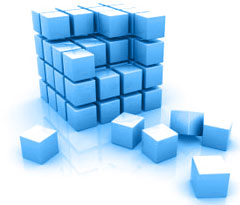
\includegraphics[width=0.8\textwidth]{./Images/modules.jpg}
            \end{center}
        \end{columns}
	\end{frame}

    \subsection{Tryton vs Odoo}

    \begin{frame}{Tryton vs Odoo}
        \fontsize{10}{11}\selectfont
%        \begin{tcolorbox}[colback=ChetwodeBlue!10,colframe=ChetwodeBlue!60]
%            \centering
%            Facilita las contribuciones de la comunidad.
%        \end{tcolorbox}

        \begin{columns}
            \column{0.7\textwidth}
            \begin{itemize}
                \item Community Open source vs Commercial Open Source. Odoo no libera todo el código.
                \item Actualizaciones gratuitas vs Necesidad de contratar el servicio para actualizar.
                \item PostgreSQL, MySQL y SQLite vs PostgreSQL.
                \item Un repositorio por módulo vs Un repositorio para todos los módulos oficiales. Un repositorio por módulo comunitario.
                \item Soporte: pequeñas empresas vs OpenERP SA.
            \end{itemize}
            \column{0.4\textwidth}
            \vspace*{-1cm}
            \begin{center}
                
\includegraphics[width=\textwidth]{./Images/Logos/tryton-name.jpg}

                
\includegraphics[width=0.3\textwidth]{./Images/vs.png}

                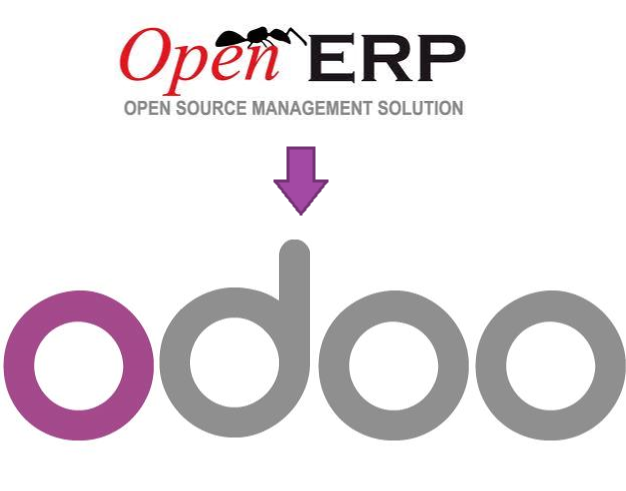
\includegraphics[width=\textwidth]{./Images/openerp-odoo.png}
            \end{center}
        \end{columns}
	\end{frame}
